\section{实验步骤}
\subsection{在 UNIX V6++中添加一个新的系统调用接口}
如图\ref{declear}-\ref{implementaion}所示,为了在UNIX V6++中添加\texttt{Sys\_Getpid}系统调用接口,我首先
向\texttt{SystemCall.h}中添加\texttt{Sys\_Getppid}的声明。
然后
在\texttt{SystemCall.cpp}中修改系统调用表中的一项,并
在\texttt{SystemCall.cpp}中实现\texttt{Sys\_Getppid}。
\begin{figure}[!htbp]
    \centering
    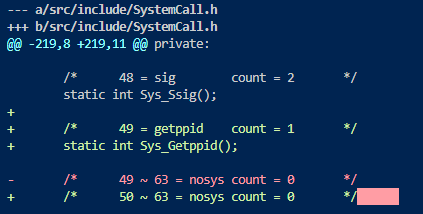
\includegraphics[scale=1]{images/declear.png}
    \caption{向\texttt{SystemCall.h}中添加\texttt{Sys\_Getppid}的声明}\label{declear}
\end{figure}

\begin{figure}[!htbp]
    \centering
    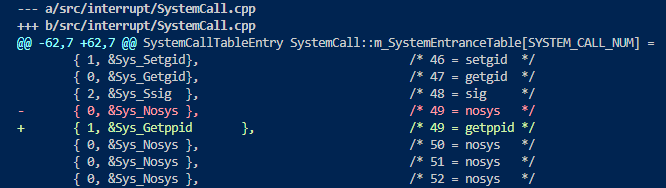
\includegraphics[width=\textwidth]{images/entry.png}
    \caption{在\texttt{SystemCall.cpp}中修改系统调用表中的一项}\label{entry}
\end{figure}

\begin{figure}[!htbp]
    \centering
    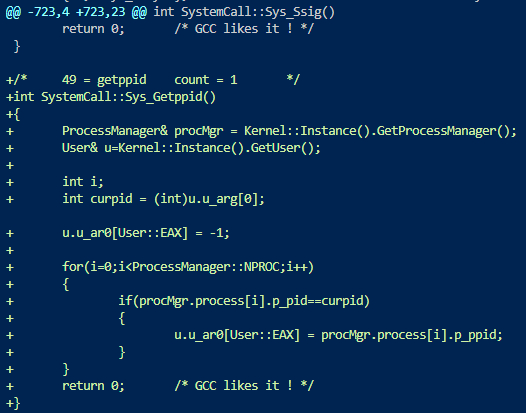
\includegraphics[scale=1]{images/implementaion.png}
    \caption{在\texttt{SystemCall.cpp}中实现\texttt{Sys\_Getppid}}\label{implementaion}
\end{figure}


\subsection{为新的系统调用添加对应的库函数并进行测试}

如图\ref{lib_declear},\ref{lib_implement}所示,为了在UNIX V6++中添加库函数的方法,我分别向\texttt{sys.h}与\texttt{sys.c}中添加了
新增库函数的声明和实现。

在库函数的实现中,\texttt{"=a"(res)}的含义是将系统调用函数返回值存放如变量\texttt{res}中;
\texttt{"a"(49)}的含义是调用第49号系统调用函数,即之前添加的\texttt{Sys\_Getppid};
\texttt{"b"(pid)}则的作用是把变量\texttt{pid}作为系统调用函数的参量传入。

\begin{figure}[!htbp]
    \centering
    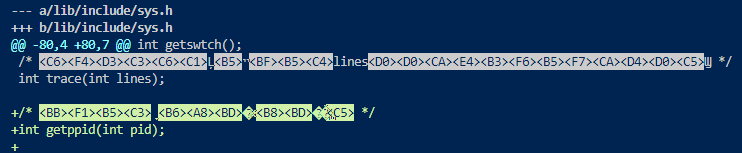
\includegraphics[width=\textwidth]{images/lib_declear.png}
    \caption{在\texttt{sys.h}中添加库函数声明}\label{lib_declear}
\end{figure}

\begin{figure}[!htbp]
    \centering
    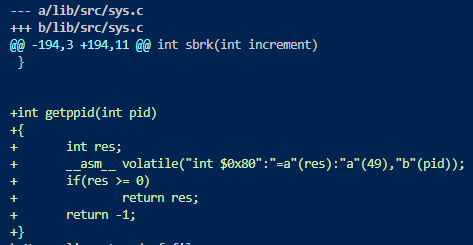
\includegraphics[scale=1]{images/lib_implement.png}
    \caption{在\texttt{sys.c}中添加库函数的实现}\label{lib_implement}
\end{figure}

为了测试之前添加的系统调用函数\texttt{Sys\_Getppid},如图\ref{test_program}所示,我在\texttt{program}文件夹下添加了\text{getppid.c}文件。

使用\texttt{make all}添加测试程序可执行文件并运行,可以得到图\ref{test}中的结果,符合预期。

\begin{figure}[!htbp]
    \centering
    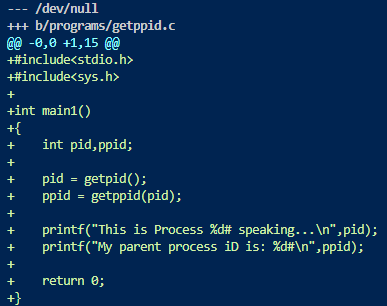
\includegraphics[scale=1]{images/test_program.png}
    \caption{在\texttt{program}文件夹下新增测试程序源文件}\label{test_program}
\end{figure}


\begin{figure}[!htbp]
    \centering
    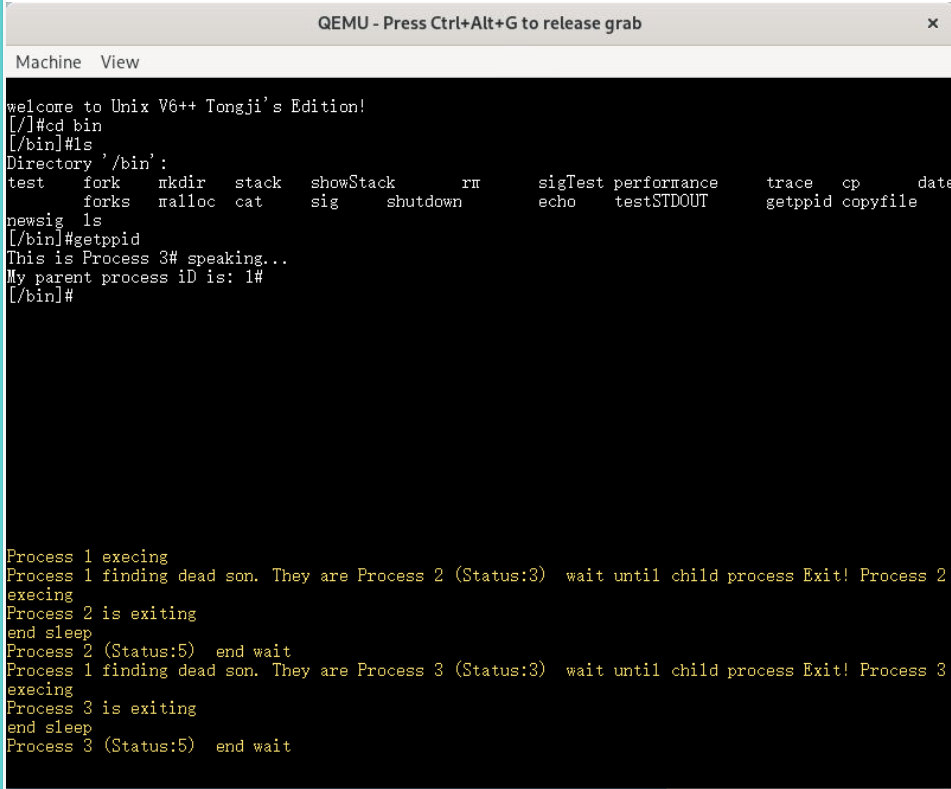
\includegraphics[width=\textwidth]{images/test.png}
    \caption{测试程序运行结果}\label{test}
\end{figure}


\subsection{调试程序}

如图\ref{getppid}所示,在\texttt{getppid}函数体内设置断点后,将调试目标设置为应用程序,
命中断点后,打开反汇编窗口,并在最近一条\texttt{int 80}语句出设置断点。点击继续,如图\ref{disammble}所示,命中\texttt{int 80}处的断点。
此时各寄存器中的值如图\ref{int80}所示。

接着,如图\ref{sys_breakpoint}所示,我在\texttt{Sys\_Getppid}体内设置两处断点。同时,我将调试目标切换至内核。
命中第一个和第二个断点时\texttt{u\_ar0}所指向的值以及\texttt{u\_arg}中存储的值如图\ref{enter}、\ref{return}所示。

\begin{figure}[!htbp]
    \centering
    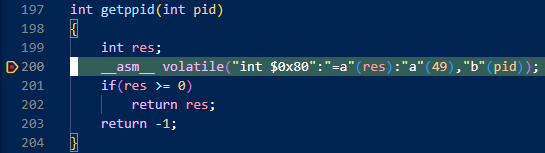
\includegraphics[scale=1]{images/getppid_breakpoint.png}
    \caption{命中getppid函数体内部的断点}\label{getppid}
\end{figure}

\begin{figure}[!htbp]
    \centering
    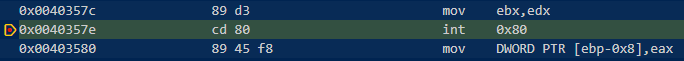
\includegraphics[width=\textwidth]{images/disammble_breakpoint.png}
    \caption{命中在int 80汇编语句处的断点}\label{disammble}
\end{figure}

\begin{figure}[!htbp]
    \centering
    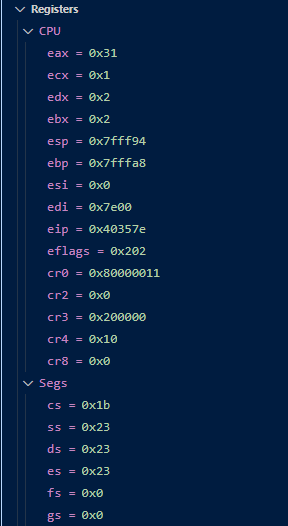
\includegraphics[scale=1]{images/int80.png}
    \caption{系统调用前各寄存器内的值}\label{int80}
\end{figure}

\begin{figure}[!htbp]
    \centering
    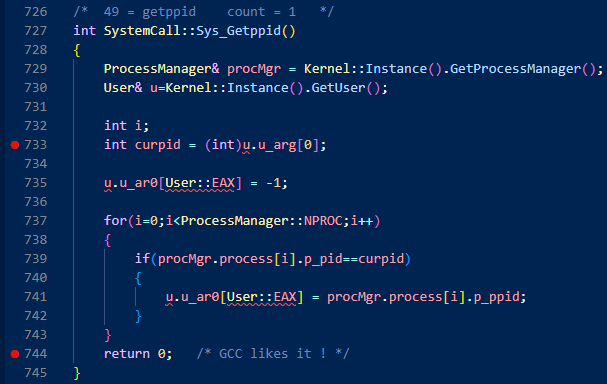
\includegraphics[width=\textwidth]{images/sys_brakpoint.png}
    \caption{在Sys\_Getppid函数体内设置断点}\label{sys_breakpoint}
\end{figure}

\begin{figure}[!htbp]
    \centering
    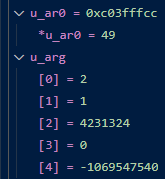
\includegraphics[scale=1]{images/enter.png}
    \caption{进入系统调用时u\_ar0所指向的值以及u\_arg中存储的值}\label{enter}
\end{figure}

\begin{figure}[!htbp]
    \centering
    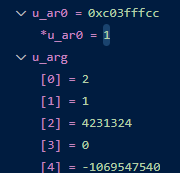
\includegraphics[scale=1]{images/return.png}
    \caption{系统调用准备好返回值时u\_ar0所指向的值以及u\_arg中存储的值}\label{return}
\end{figure}

为了观察系统调用过程中核心栈的变化,除了图\ref{sys_breakpoint}中的两处断点外,我还在线性查找循环启动处设置断点,并视察命中这些断点时\texttt{0xC03FFFCC}附近的内存单元。

在图\ref{sys_breakpoint}中的第一个断点处,运行命令\texttt{exec x /32xw 0xC03FFF8C}得到的结果如图\ref{mem1}所示。

\newpage

\begin{Verbatim}[frame=single,fontsize=\small]
    -exec x /60xw 0xC03FFF1C
    0xc03fff1c:	0xc011c9e0	0xc0202000	0xc03fff44	0xc0108017
    0xc03fff2c:	0x00000002	0xc03ff000	0xc0120aa0	0xc010759f
    0xc03fff3c:	0xc011c9e0	0x00000400	0xc03fff64	0xc01075cc
    0xc03fff4c:	0x00000020	0x00000020	0xc03fff94	0xc03ff000
    0xc03fff5c:	0x00000020	0x00000002	0xc03fff94	0xc01074e1
    0xc03fff6c:	0xc0107ff8	0xc0202000	0xc03fff94	0xc01073df
    0xc03fff7c:	0xc0117f48	0xc03ff000	0x00000001	0xc03fffb8
    0xc03fff8c:	0xc011c9e0	0x00109a97	0xc03fffe8	0xc0107360
    0xc03fff9c:	0xc03fffa4	0xc03fffec	0x00000000	0x00000000
    0xc03fffac:	0x00000023	0x00000023	0x00000002	0x00000001
    0xc03fffbc:	0x00000002	0x00000000	0x00007e00	0xc03fffe8
    0xc03fffcc:	0x00000031	0x00000001	0xc03ff000	0xc0124984
    0xc03fffdc:	0xc03fffec	0xc0007e00	0xc0007e00	0x007fffa8
    0xc03fffec:	0x00403580	0x0000001b	0x00010202	0x007fff94
    0xc03ffffc:	0x00000023	Cannot access memory at address 0xc0400000
\end{Verbatim}
\captionof{figure}{进入系统调用时u\_ar0所指内存地址附近的内存单元}\label{mem1}

在线性查找循环开始处,运行命令\texttt{exec x /32xw 0xC03FFF8C}得到的结果如图\ref{mem2}所示。

\begin{Verbatim}[frame=single,fontsize=\small]
    -exec x /60xw 0xC03FFF1C
    0xc03fff1c:	0xc011c9e0	0xc0202000	0xc03fff44	0xc0108017
    0xc03fff2c:	0x00000002	0xc03ff000	0xc0120aa0	0xc010759f
    0xc03fff3c:	0xc011c9e0	0x00000400	0xc03fff64	0xc01075cc
    0xc03fff4c:	0x00000020	0x00000020	0xc03fff94	0xc03ff000
    0xc03fff5c:	0x00000020	0x00000002	0xc03fff94	0xc01074e1
    0xc03fff6c:	0xc0107ff8	0xc0202000	0xc03fff94	0xc01073df
    0xc03fff7c:	0xc0117f48	0xc03ff000	0x00000001	0xc03fffb8
    0xc03fff8c:	0xc011c9e0	0x00109a97	0xc03fffe8	0xc0107360
    0xc03fff9c:	0xc03fffa4	0xc03fffec	0x00000000	0x00000000
    0xc03fffac:	0x00000023	0x00000023	0x00000002	0x00000001
    0xc03fffbc:	0x00000002	0x00000000	0x00007e00	0xc03fffe8
    0xc03fffcc:	0xffffffff	0x00000001	0xc03ff000	0xc0124984
    0xc03fffdc:	0xc03fffec	0xc0007e00	0xc0007e00	0x007fffa8
    0xc03fffec:	0x00403580	0x0000001b	0x00010202	0x007fff94
    0xc03ffffc:	0x00000023	Cannot access memory at address 0xc0400000
\end{Verbatim}
\captionof{figure}{进入系统调用时u\_ar0所指内存地址附近的内存单元}\label{mem2}

在图\ref{sys_breakpoint}的第二个断点处,运行命令\texttt{exec x /32xw 0xC03FFF8C}得到的结果如图\ref{mem3}所示。

\begin{Verbatim}[frame=single,fontsize=\small]
    -exec x /60xw 0xC03FFF1C
    0xc03fff1c:	0xc03fff44	0xc0108042	0x00000008	0x00010282
    0xc03fff2c:	0x00000002	0xc03ff000	0xc0120aa0	0x00000064
    0xc03fff3c:	0xc011c9e0	0x00000400	0xc03fff64	0xc01075cc
    0xc03fff4c:	0x00000020	0x00000020	0xc03fff94	0xc03ff000
    0xc03fff5c:	0x00000020	0x00000002	0xc03fff94	0xc01074e1
    0xc03fff6c:	0xc0107ff8	0xc0202000	0xc03fff94	0xc01073df
    0xc03fff7c:	0xc0117f48	0xc03ff000	0x00000001	0xc03fffb8
    0xc03fff8c:	0xc011c9e0	0x00109a97	0xc03fffe8	0xc0107360
    0xc03fff9c:	0xc03fffa4	0xc03fffec	0x00000000	0x00000000
    0xc03fffac:	0x00000023	0x00000023	0x00000002	0x00000001
    0xc03fffbc:	0x00000002	0x00000000	0x00007e00	0xc03fffe8
    0xc03fffcc:	0x00000001	0x00000001	0xc03ff000	0xc0124984
    0xc03fffdc:	0xc03fffec	0xc0007e00	0xc0007e00	0x007fffa8
    0xc03fffec:	0x00403580	0x0000001b	0x00010202	0x007fff94
    0xc03ffffc:	0x00000023	Cannot access memory at address 0xc0400000
\end{Verbatim}
\captionof{figure}{系统调用准备好返回值时u\_ar0所指内存地址附近的内存单元}\label{mem3}

结合图\ref{mem1}-\ref{mem3}以及图\ref{stack}中的调用栈,我们可以得到表\ref{table2}和图\ref{3vs2},\ref{2vs1}及其分析。

\begin{figure}[!htbp]
    \centering
    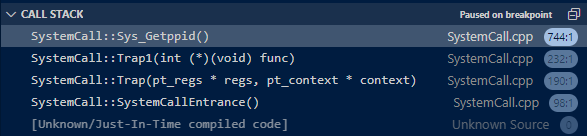
\includegraphics[scale=1]{images/stack.png}
    \caption{程序在\texttt{Sys\_Getppid}内部时的调用栈}\label{stack}
\end{figure}
